\documentclass[8pt,a4paper,landscape]{scrartcl} 
\usepackage[left=1cm,right=1cm,top=1cm,bottom=1cm,landscape]{geometry} 
\usepackage[utf8]{inputenc} 
\usepackage[ngerman]{babel} 
\usepackage{multicol} 
\usepackage{lipsum}
\usepackage{amsmath} 
\usepackage{amsfonts} 
\usepackage{amssymb} 
\usepackage{gensymb} 
\usepackage{dsfont} 
\usepackage{calc} 
\usepackage{tabularx}
\usepackage[table]{xcolor}
\usepackage{arydshln}
\usepackage{tikz}
\usepackage{multirow}
\usetikzlibrary{calc,arrows}
%\usepackage[permil]{overpic} \usepackage{graphicx} \graphicspath{{gfx/}} 

\definecolor{Gray}{gray}{0.9}
\definecolor{LightCyan}{rgb}{0.88,1,1}


\newcolumntype{Y}{>{\centering\arraybackslash}X}
\renewcommand\tabularxcolumn[1]{m{#1}}% for vertical centering text in X column
\renewcommand{\arraystretch}{1.25}
\renewcommand{\arraycolsep}{1.25pt}
\newcommand{\tikzmark}[1]{%
	\tikz[overlay,remember picture] \node (#1) {};}


\author{Levin Baumann} 



\title{Formelsammlung Robotik} 

\begin{document} 
\setlength{\columnsep}{1cm} 
\begin{multicols*}{3}
{\LARGE\bfseries Formelsammlung Robotik }

\subsection*{Vektoren}
\subsubsection*{Mathematische Operationen im Vektorraum}
\renewcommand{\arraystretch}{1}
\begin{tabularx}{\columnwidth}{l|c|X}
	Addition & $\vec{a} + \vec{b}$ & 
	$\left(\begin{array}{c}                         a_1 + b_1 \\
	a_2 + b_2 \\
	a_3 + b_3 \\                               
	\end{array}\right)$ \\ \hline
	Subtraktion & $\vec{a}-\vec{b}$ & 
	$\left(\begin{array}{rrr}                       a_1 - b_1\\
	a_2 - b_2\\
	a_3 - b_3\\                 
	\end{array}\right)$ \\ \hline
	Skalare Multipl. & $ \lambda \cdot \vec{a}$ & 
	$\left(\begin{array}{rrr}                       \lambda \cdot a_1\\
	\lambda \cdot a_2\\
	\lambda \cdot a_3\\                 
	\end{array}\right)$\\ \hline
	Abstand P.-Urpsr. & \\
	Betrag (Norm) & $ ||\vec{a}||$ & 
	$|\vec{a}| = \sqrt{{a_1}^2 + {a_2}^2 + {a_3}^2}$\\ \hline
	Skalarprodukt & $\vec{a}\cdot\vec{b}$ & $a_1 \cdot b_1 + \ldots + a_n \cdot b_n = x$ \\ \hline
	Kreuzprodukt & $\vec{a} \times \vec{b}$ &$\left(\begin{array}{c}                         a_2 \cdot b_3 - a_3 \cdot b_2 \\
	a_3 \cdot b_1 - a_1 \cdot b_3 \\
	a_1 \cdot b_2 - a_2 \cdot b_1 \\                               
	\end{array}\right)$ \\ \hline
	Spatprodukt & $u \cdot (v \times w)$ & $\left|\begin{array}{ccc}
		 u_1  &  u_2  &  u_3  \\
		 v_1  &  v_2  &  v_3  \\
		 w_1  &  w_2  &  w_3  \\
	\end{array}\right|$ (siehe Determinante) \\ \hline
	Winkel &  & $\cos \alpha = \dfrac{\vec{a} \cdot \vec{b}}{|\vec{a}| \cdot |\vec{b}|}$ \\ \hline
	Rotationsmatrix & & $\left(\begin{Array}{ll}
	\cos \alpha & -\sin \alpha\\
	\sin \alpha & \cos \alpha\\
	\end{Array}\right) \cdot \left(\begin{Array}{c}
	x
	\\
	y
	\end{Array}\right)$
\end{tabularx}

\subsection*{Matrizen}
\subsubsection*{Operatoren}
\begin{tabularx}{\columnwidth}{r|c|X}
	Gleich & $ A = B $ & $ \left(a_{ij}\right) = \left(b_{ij}\right)$ \\ \hline
	Addition & $ C = A + B $ & $ \left(c_{ij}\right) = \left(a_{ij}\right) + \left(b_{ij}\right) $ \\ \hline
	Differenz & $ C = A - B $ &  $ \left(c_{ij}\right) = \left(a_{ij}\right) - \left(b_{ij}\right) $ \\ \hline
	Multiplikation Skalar & $ c \cdot A $ & $ cA \in R^{m \times n} $ \\ \hline
	Multiplikation Matrizen & $ A \cdot B $ & $ AB = \sum_{j} a_{ij}b_{ij} $
\end{tabularx}
%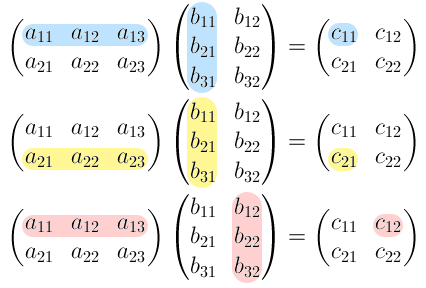
\includegraphics[width=\columnwidth]{mmultipl}

\subsubsection*{Multiplikation}

	$\left(\begin{Array}{ccc}
	\rowcolor{blue!20}
		a_{11} & a_{12} & a_{13}\\
		a_{21} & a_{22} & a_{23}\\
	\end{Array}\right)
	\cdot
	\left(\begin{Array}{>{\columncolor{blue!20}}cc}
	b_{11} & b_{12}\\
	b_{21} & b_{22}\\
	b_{31} & b_{32}
	\end{Array}\right)
	= 
	\left(\begin{Array}{cc}
	\cellcolor{blue!20} a_{11} \cdot b_{11} + a_{12} \cdot b_{21} + a_{13} \cdot b_{31} & c_{12}\\
	c_{21} & c_{22}
	\end{Array}\right)
	$\\
	$\left(\begin{Array}{ccc}
	\rowcolor{red!20}
	a_{11} & a_{12} & a_{13}\\
	a_{21} & a_{22} & a_{23}\\
	\end{Array}\right)
	\cdot
	\left(\begin{Array}{c>{\columncolor{red!20}}c}
	b_{11} & b_{12}\\
	b_{21} & b_{22}\\
	b_{31} & b_{32}
	\end{Array}\right)
	= 
	\left(\begin{Array}{cc}
	c_{11} & \cellcolor{red!20} c_{12}\\
	c_{21} & c_{22}
	\end{Array}\right)
	$\\
	$\left(\begin{Array}{ccc}
		a_{11} & a_{12} & a_{13}\\
		\rowcolor{yellow!50}
		a_{21} & a_{22} & a_{23}\\
	\end{Array}\right)
	\cdot
	\left(\begin{Array}{>{\columncolor{yellow!50}}cc}
		b_{11} & b_{12}\\
		b_{21} & b_{22}\\
		b_{31} & b_{32}
	\end{Array}\right)
	= 
	\left(\begin{Array}{cc}
		c_{11} & c_{12}\\
		\cellcolor{yellow!50} c_{21} & c_{22}
	\end{Array}\right)
	$\\

\subsubsection*{Inverse bilden}
\begin{tabularx}{\columnwidth}{rcl}
& & $A \cdot A ^{-1} = I | A=(a_{ij}), A^{-1} = (a_{ij})$\\
\multicolumn{3}{l}{Multiplikation aus $A$ und $A^{-1}$ ergeben Einheitsmatrix:}\\
& & $
\left(\begin{Array}{ccc}
a_{11} & \dots & a_{1n}\\
\vdots &       & \vdots\\
a_{n1} & \dots & a_{nn}\\
\end{Array}\right)
\cdot
\left(\begin{array}{ccc}
\hat{a}_{11} & \dots & \hat{a}_{1n} \\
\vdots    &       &    \vdots    \\
\hat{a}_{n1} & \dots & \hat{a}_{nn}
\end{array}\right)
=
\left(\begin{Array}{ccc}
1 &        & 0\\
& \ddots &  \\
0 &        & 0\\
\end{Array}\right)
$\\
\multicolumn{3}{l}{Inverse kann mit Gauß-Jordan berechnet werden.}\\
\multicolumn{3}{l}{Koeffizientenmatrix $A$ umd Einheitsmatrix $I$ erweitern.}\\
$(A|I)$ & $=$ & $\left(\begin{Array}{ccc|ccc}
a_{11} & \dots & a_{1n} & 1 &        & 0\\
\vdots &       & \vdots &   & \ddots &  \\
a_{n1} & \dots & a_{nn} & 0 &        & 0\\
\end{Array}\right)$ \\
\multicolumn{3}{l}{Matrix $A$ mit elementarer Zeilenumformung auf obere Dreiecksgestalt}\\
\multicolumn{3}{l}{bringen, wobei Einheitsmatrix $I$ mit umgeformt wird:} \\ 
$(D|B)$ & $=$ & $\left(\begin{array}{ccc|ccc}
	\ast & \dots  &  \ast  &  \ast  & \dots &  \ast  \\
	     & \ddots & \vdots & \vdots &       & \vdots \\
	 0   &        &  \ast  &  \ast  & \dots &  \ast
\end{array}\right)$ \\
\multicolumn{3}{l}{Matrix $A$ ist nur invertierbar, wenn $D$ keine Null auf Hauptdiagonale}\\
\multicolumn{3}{l}{$D$ mit elementarer Zeilenumformung auf Diagonalgestalt und durch}\\
\multicolumn{3}{l}{Skalierung in Einheitsmatrix. Rechte Seite enthält die Inverse.}\\
$(I|A^{-1})$ & $=$ & $\left(\begin{array}{ccc|ccc}
	1 &        & 0 & \hat{a}_{11} & \dots & \hat{a}_{1n} \\
	  & \ddots &   &    \vdots    &       &    \vdots    \\
	0 &        & 1 & \hat{a}_{n1} & \dots & \hat{a}_{nn} \\
\end{array}\right)$
\end{tabularx}

\subsubsection*{Rechte Hand Regel}
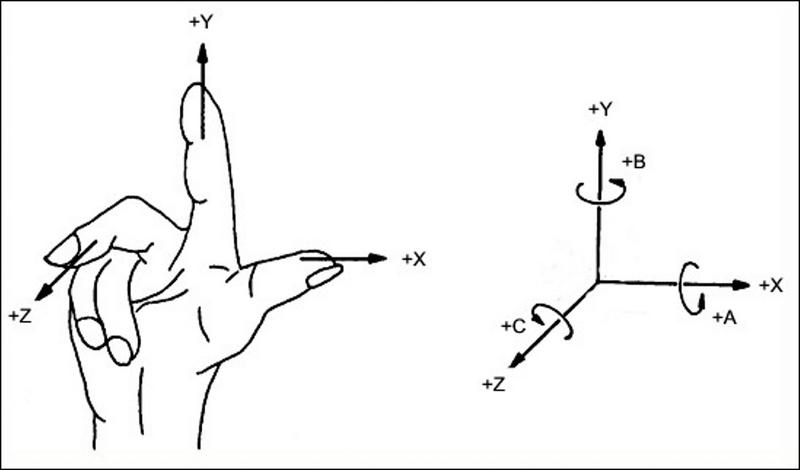
\includegraphics[width=.9\columnwidth]{rechteHand.jpg}
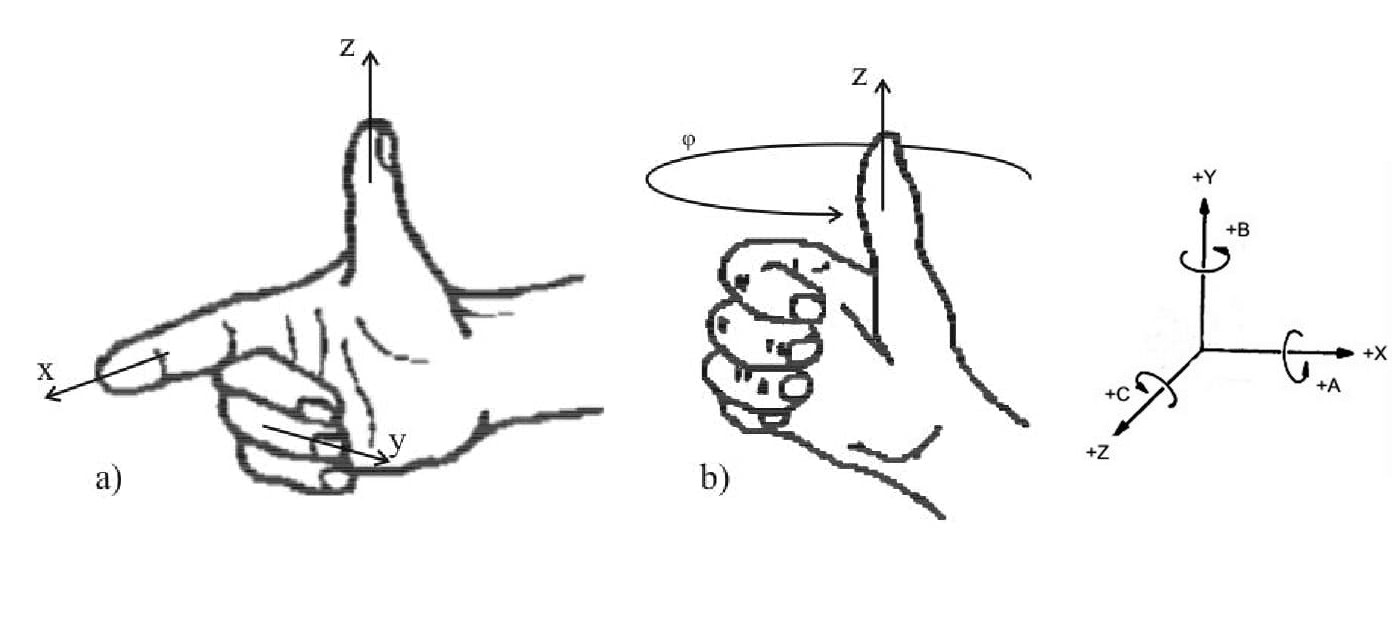
\includegraphics[width=.9\columnwidth]{handRotation.jpg}

\subsection*{Koordinatensysteme}
\begin{tabularx}{\columnwidth}{l|X|c}
	Objekt in 3D (OKS) & $\vec{v} = (x,y,z,\alpha,\beta,\gamma)$ & $\alpha,\beta,\gamma = $ Drehwinkel \\ \hline
	Senkrechte &  \\ 
	
\end{tabularx}

\subsection*{Rotationsmatrizen}
\begin{tabularx}{\columnwidth}{X|p{.8\columnwidth}}
	Rotation um X & $R_x(\alpha) = \left[\begin{Array}{c} x' \\ y' \\ z' \end{Array}\right]
	= \left[\begin{Array}{ccc}
		1 & 0 & 0\\
		0 & \cos\alpha & -\sin\alpha\\
		0 & \sin\alpha & \cos\alpha
	\end{Array}\right]\cdot\left[\begin{Array}{c}
		x\\
		y\\
		z
	\end{Array}\right]$\\ \hline
Rotation um Y & $R_y(\alpha) = \left[\begin{Array}{c} x' \\ y' \\ z' \end{Array}\right]
= \left[\begin{Array}{ccc}
	\cos\alpha & 0 & \sin\alpha\\
	0 & 1 & 0 \\
	-\sin\alpha & 0 & \cos\alpha
\end{Array}\right]\cdot\left[\begin{Array}{c}
	x\\
	y\\
	z
\end{Array}\right]$\\ \hline
Rotation um Z & $R_z(\alpha) = \left[\begin{Array}{c} x' \\ y' \\ z' \end{Array}\right]
= \left[\begin{Array}{ccc}
	\cos\alpha & -\sin\alpha & 0\\
	\sin\alpha & \cos\alpha & 0\\
	0 & 0 & 1
\end{Array}\right]\cdot\left[\begin{Array}{c}
	x\\
	y\\
	z
\end{Array}\right]$\\ \hline
\multicolumn{1}{p{.2\columnwidth}|}{Vormultipl.\newline(Roll-pitch-yaw)} & Rotation um die ursprüngliche (feste) Achse. Schreibweise: Letzte Drehung $\rightarrow$ 1. Drehung\\ \hline
\multicolumn{1}{p{.2\columnwidth}|}{Nachmultipl.\newline (Euler-Winkel)} & Rotation um die neuen (momentanen) Achsen. Schreibweise: 1. Drehung $\rightarrow$ Letzte Drehung\\ \hline
Homogene $4\times4$-Matrix & $T = \left(\begin{Array}{c|c}
	R_{3\times3} & u_{3\times1}\\ \hline
	f_{1\times3} = 0 & 1\times1
\end{Array}\right) = \left(\begin{Array}{cccc}
n_{x\downarrow z} & o_{x\downarrow z} & a_{x\downarrow z} & u_{x\downarrow z}\\
0 & 0& 0 & 1
\end{Array}\right)$\\ \hline
Invertierung 4$\times$4 &  $T^{-1} = \left(\begin{Array}{ccc:c}
	n_{x} & n_{y} & n_{z} & -n^{T}\cdot\vec{u}\\
	o_{x} & o_{y} & o_{z} & -o^{T}\cdot\vec{u}\\
	a_{x} & a_{y} & a_{z} & -a^{T}\cdot\vec{u}\\ \cdashline{1-3}
	0 & 0&0&1
\end{Array}\right)$\\ \hline
Verkettete Lagebeschr.-& $ ^{BKS}H_{B}  = ^{BKS}H_{A} \cdot ^{A}H_{B} | H = \text{Homogene Matr.} $\\ \hline
test&

\end{tabularx}


\end{multicols*}
\end{document}